\section{Discussion}
Because the Discussion section will often refer back to the results, it is useful to take advantage of cross-referencing (see Table~\ref{tab:RTmeans}). 

Sometimes the discussion section may even include additional figures.  If the figures are small enough and you don't want them to take up the full line, you can always use the \texttt{wrapfigure} environment.

\begin{wrapfigure}{l}{0.4\textwidth}     \centering       
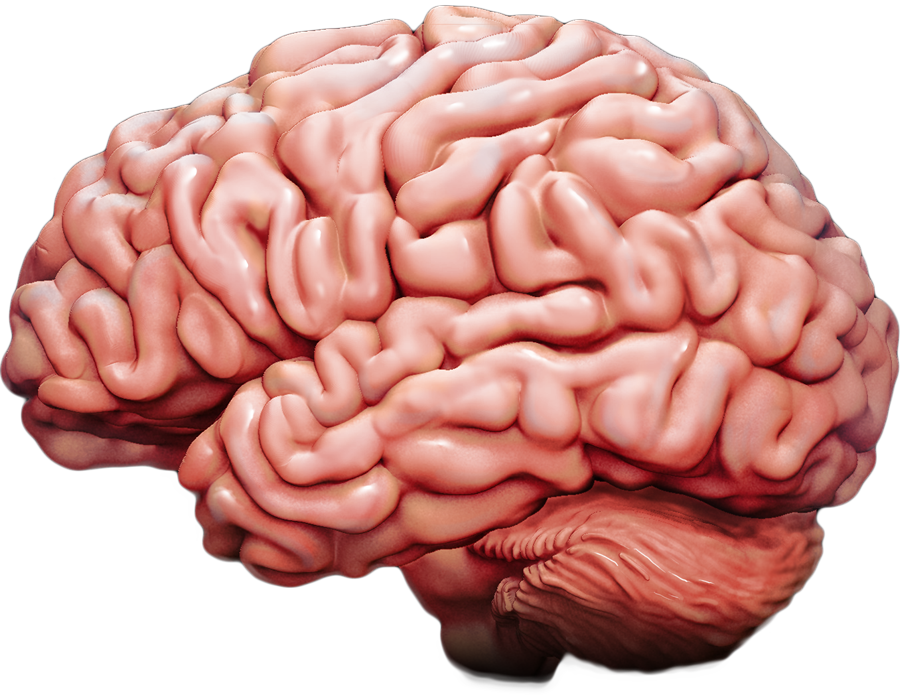
\includegraphics[width=0.25\textwidth]{brain-lateral.png}
\caption{\label{fig:latbrain} Yet another figure caption here.}
\end{wrapfigure}

Figure~\ref{fig:gearhead} was also a great example for the Results right? But what if you have a small figure and you just want to wrap the text neatly around it?  Never fear....the ``wrapfig'' package is here! The wrapfig environment allows you to neatly wrap text around your figures just like the journals do. \blindtext
